\chapter{MARCO TEÓRICO}

En el presente capítulo se realizará una exploración de los conceptos
necesarios a fin de desarrollar el módulo de teleoperación con feedback
háptico. En primer lugar, se aborda un acercamiento al ámbito médico dentro del
campo de la robótica en cirugías. Asimismo, se explica la estructura de un
sistema háptico y las distintas técnicas de aplicación existentes. Por otro
lado, se detallan las teorías de diseño cinemático y dinámico en un
manipulador, como es el caso del robot UR5. Además, se describe el método de
control aplicado en el sistema y las ecuaciones necesarias para su
implementación. Por último, se presenta el marco de trabajo del Sistema
Operativo Robótico (ROS) empleado para la integración del sistema, junto con
las herramientas gráficas (Rviz, Gazebo y Qt5) utilizadas para la
visualización y el desarrollo de la interfaz de usuario.

\section{Contexto del procedimiento de sutura externa y requerimientos para
  teleoperación}
Una herida cutánea o externa, desde su generación hasta su cierre, presenta 3
etapas previas a su curación. La Fase inflamatoria, donde se empieza la
coagulación de la herida; la fase proliferativa, donde se crean nuevos tejidos
que cubrirán la herida, y la fase de remodelación, donde la herida termina de
cicatrizar \cite{Cicatritacion}. El tiempo de duración de cada etapa dependerá
de la naturaleza de la herida y su condición al momento de la revisión. Tomando
estos factores en cuenta se puede determinar si es necesario asegurar la
conclusión de alguna de las fases mencionadas con una sutura o si, por el
contrario, solo desinfectar la zona afectada.

Para los casos de aplicación de suturas, es considerada en el campo médico como
el material encargado del cierre de heridas~\cite{GONZALEZ-CELY2018}. De este
modo, las suturas enfocadas en heridas superficiales se considerarían como
suturas externas. El proceso de suturar es el acercamiento de tejidos separados
productos de un corte para su correcta cicatrización. Tomando en cuenta el área
afectada, puede necesitarse hilos especiales  e instrumental quirúrgico
adicional~\cite{GONZALEZ-CELY2018}.

\subsection{Herramientas comunes}
Dentro de las herramientas básicas para realizar una sutura se encuentra el
porta agujas, la pinza, tijeras y el bisturí. Además de estos, se debe
complementar con anestésico local.

\begin{figure}[H]
    \centering
    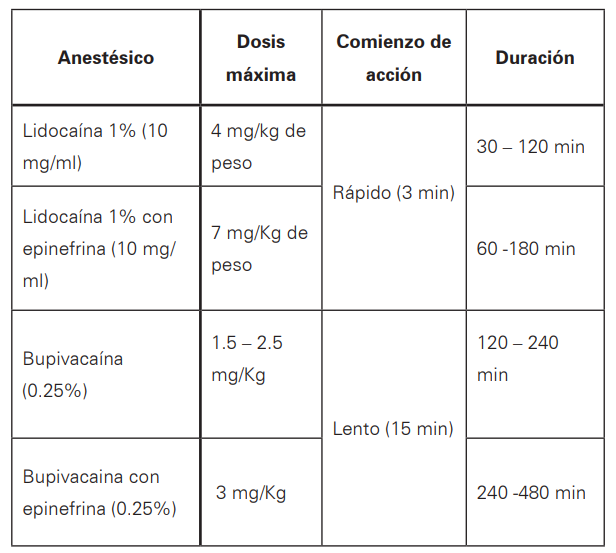
\includegraphics[width=0.75\linewidth]{images/anastesicos.png}
    \caption{Anestésicos locales más utilizados\cite{GONZALEZ-CELY2018}}
    \label{fig:enter-label}
\end{figure}

\subsection{Características a considerar}
Dentro de las características más importantes, está el material de la
sutura. Como se describió a principios del capítulo, la sutura también es la
denominación del material con el que se realiza el cierre de la herida;
pudiendo ser hilos, grapas, bandas adhesivas, etc. Su elección dependerá del
tiempo de permanencia requerido y del área a suturar.

Para el caso del uso de hilos, el calibre y el tiempo de permanencia del
hilo utilizado variará dependiendo del área anatómica a suturar, por ejemplo,
una área de alto movimiento, como una articulación, necesitará un tiempo más
prolongado. Asimismo, el material del hilo variará dependiendo de la aplicación
y condiciones de la piel.

\begin{figure}[H]
    \centering
    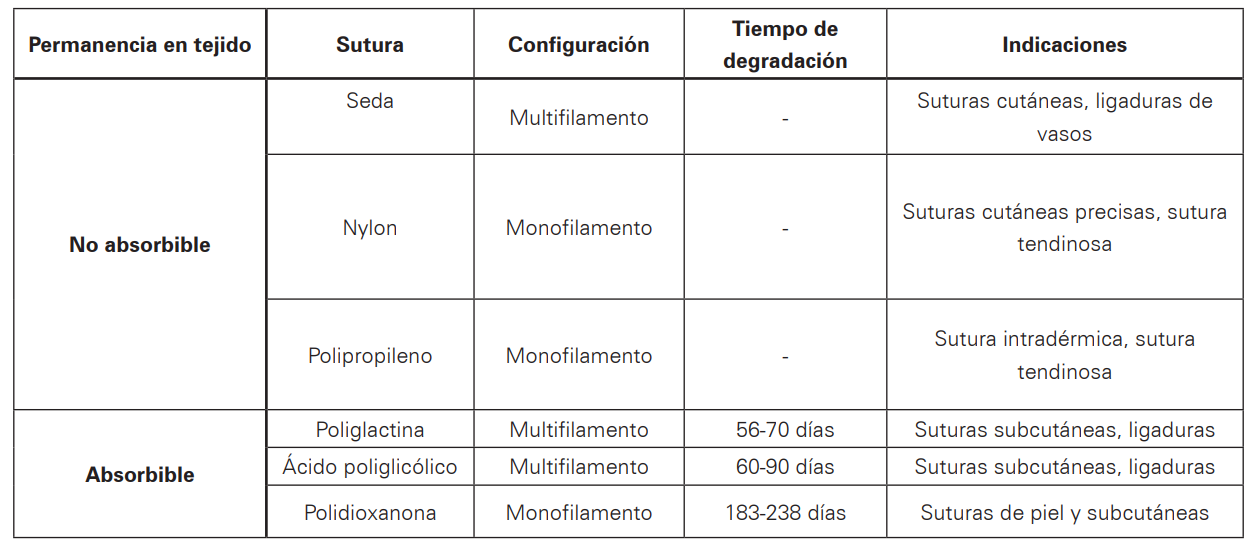
\includegraphics[width=1\linewidth]{images/hilos.png}
    \caption{Tipos de hilos en suturas\cite{GONZALEZ-CELY2018}}
    \label{fig:enter-label}
\end{figure}

\subsection{Técnicas de aplicación de suturas}
\textbf{Pasos para realizar una sutura}:
\begin{enumerate}
    \item Limpieza y desinfección de la herida.
    \item Aplicación anestesia local.
    \item Cierre de la herida con sutura de hilo.
    \item Nudo para con doble lazada y luego lazadas
          simples\cite{GONZALEZ-CELY2018}
    \item Cubrir área suturada.
\end{enumerate}

% %explicar la teoria presente en libros
% \section{Método de sutura robótica} %metodologia

% La sutura realizada por robots es crítico al momento de dar por finalizado un proceso quirurgico, su aplicación en laparoscopia 

\section{Teleoperación maestro–esclavo con retroalimentación háptica}

\subsection{Esquema bilateral y mapeo maestro–esclavo}

En un esquema de teleoperación bilateral, el dispositivo maestro (el Geomagic
Touch) y el manipulador esclavo (el UR5) intercambian continuamente
información de posición y de fuerza: el maestro envía la referencia de
movimiento generada por el operador, mientras que el esclavo retorna una
estimación de las fuerzas de contacto percibidas en el entorno de trabajo.
% Pendiente: detallar el mapeo específico entre la pose del Geomagic Touch y
% el espacio de trabajo del UR5 empleado en este proyecto.

\begin{figure}[H]
    \centering
    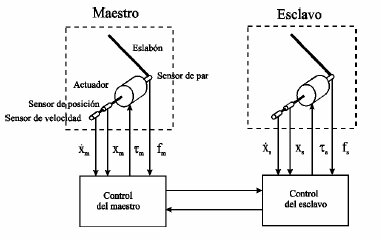
\includegraphics[width=0.75\linewidth]{images/Figura-15-Control-maestro-esclavo_W640.jpg}
    \caption{Esquema de teleoperación bilateral de cinemática proporcional~\cite{teleoperation_bilateral}}
    \label{fig:esquema_bilateral}
\end{figure}

\subsection{Escalamiento de movimiento y de fuerza}

Dado que el espacio de trabajo del Geomagic Touch es considerablemente más
reducido que el del UR5, resulta necesario definir factores de escala que
relacionen el desplazamiento del dispositivo háptico con el del efector final
del manipulador, así como un escalamiento equivalente para la fuerza
percibida por el operador.
% Pendiente: especificar los factores de escala de posición y de fuerza
% utilizados en la implementación de este proyecto.

\subsection{Principios de Funcionamiento de la Retroalimentación Háptica en
    Robótica}

El sentido del tacto es uno de los más importantes para la extracción de
características físicas de los objetos que se encuentran en el entorno y se
manipulan, ya que permite identificar la dureza y la rugosidad
\cite{El_sentido_del_tacto_revision}. De esta forma, combinando la
retroalimentación de los otros sentidos, el ser humano es capaz de comprender
lo que está manipulando. Es por esto que la parte háptica es necesaria para
mejorar la capacidad de acción del ser humano \cite{spence_gallace_touch}.
Dentro del ámbito de la sutura, es muy importante la noción de las
características físicas del tejido que se está manipulando, ya que de ello
dependerá que el método aplique más o menos fuerza al dispositivo de control
para realizar la incisión de la aguja o el agarre de la piel para mantener
estable el área que se desea perforar. En caso contrario, existe un alto riesgo
de dañar los tejidos únicamente basándose en la vista, lo que podría llevar a
consecuencias fatales para el paciente durante la operación.

% De este modo, el dispositivo háptico que se utilizará para esta investigación será capaz de transmitir únicamente la información física relacionada con la rigidez del objeto, es decir, la fuerza que opone resistencia del objeto a ser deformado. De esta forma, para el dispositivo háptico deberá ser capaz de transmitir fuerza en un espacio tridimensional. De está forma, el medico será capaz de recibir una retroalimentación de rigidez en cualquier dirección lo que mejorará su acionar al evitar ejercer más fuerza de la debida. Asimismo, el dispositivo transmitirá la fuerza por consecuencia del control de motores internos al sistema de control que usará el cirujano, ya que se buscará que estos imiten la rigidez que se está sensando al final del brazo manipulador. 

\subsection{Caracterización Técnica del Geomagic Touch}

\begin{figure}[H]
    \centering
    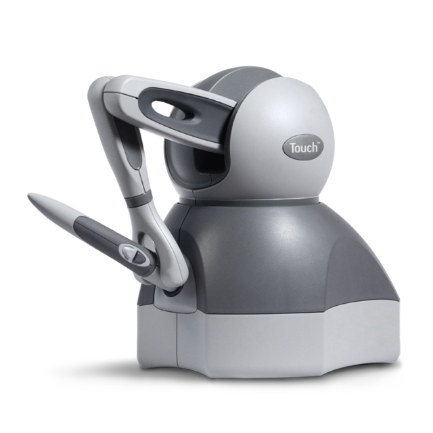
\includegraphics[width=0.75\linewidth]{encabezados/geomagic_touch.png}
    \caption{Dispositivo háptico Geomagic touch de 3D Systems}
    \label{fig:Geomagic_touch_base}
\end{figure}

El dispositivo háptico utilizado para el trabajo de investigación es el
Geomagic Touch de la empresa 3D Systems, el cual desempeña el papel de
dispositivo maestro dentro del esquema de teleoperación bilateral, mientras
que el robot UR5 actúa como manipulador esclavo. Este dispositivo cuenta con
6 grados de libertad, de los cuales la totalidad es leída mediante encoders,
aunque solamente 3 se encuentran actuados. Dado que es el robot esclavo quien
entra en contacto directo con el tejido durante la manipulación, es este el
que detecta la fuerza de interacción resultante, misma que es transmitida de
vuelta al dispositivo háptico para que este la reproduzca sobre el usuario a
través de sus 3 articulaciones actuadas. Para generar dicha
retroalimentación, el propio dispositivo estima internamente la posición y
orientación de su gripper y calcula la velocidad que deben alcanzar sus
motores con el fin de producir el estímulo de fuerza correspondiente sobre la
mano del operador. Asimismo, el dispositivo puede proyectar hasta 3.3N de
fuerza nominal para transmitir el estímulo de rigidez percibido por el
usuario al mando del sistema de control. Esta limitante deberá considerarse
frente al rango de fuerza de accionamiento requerido en el robot esclavo, el
cual puede exceder la capacidad del dispositivo háptico dada la extensión de
movimiento que podría demandar la manipulación del hilo y la aguja al suturar
el área deseada. Finalmente, el dispositivo
se comunica a una frecuencia de 1000 Hz, lo cual será determinante para
definir el periodo al que podrá actualizarse la ley de control de los
motores.

\begin{figure}[H]
    \centering
    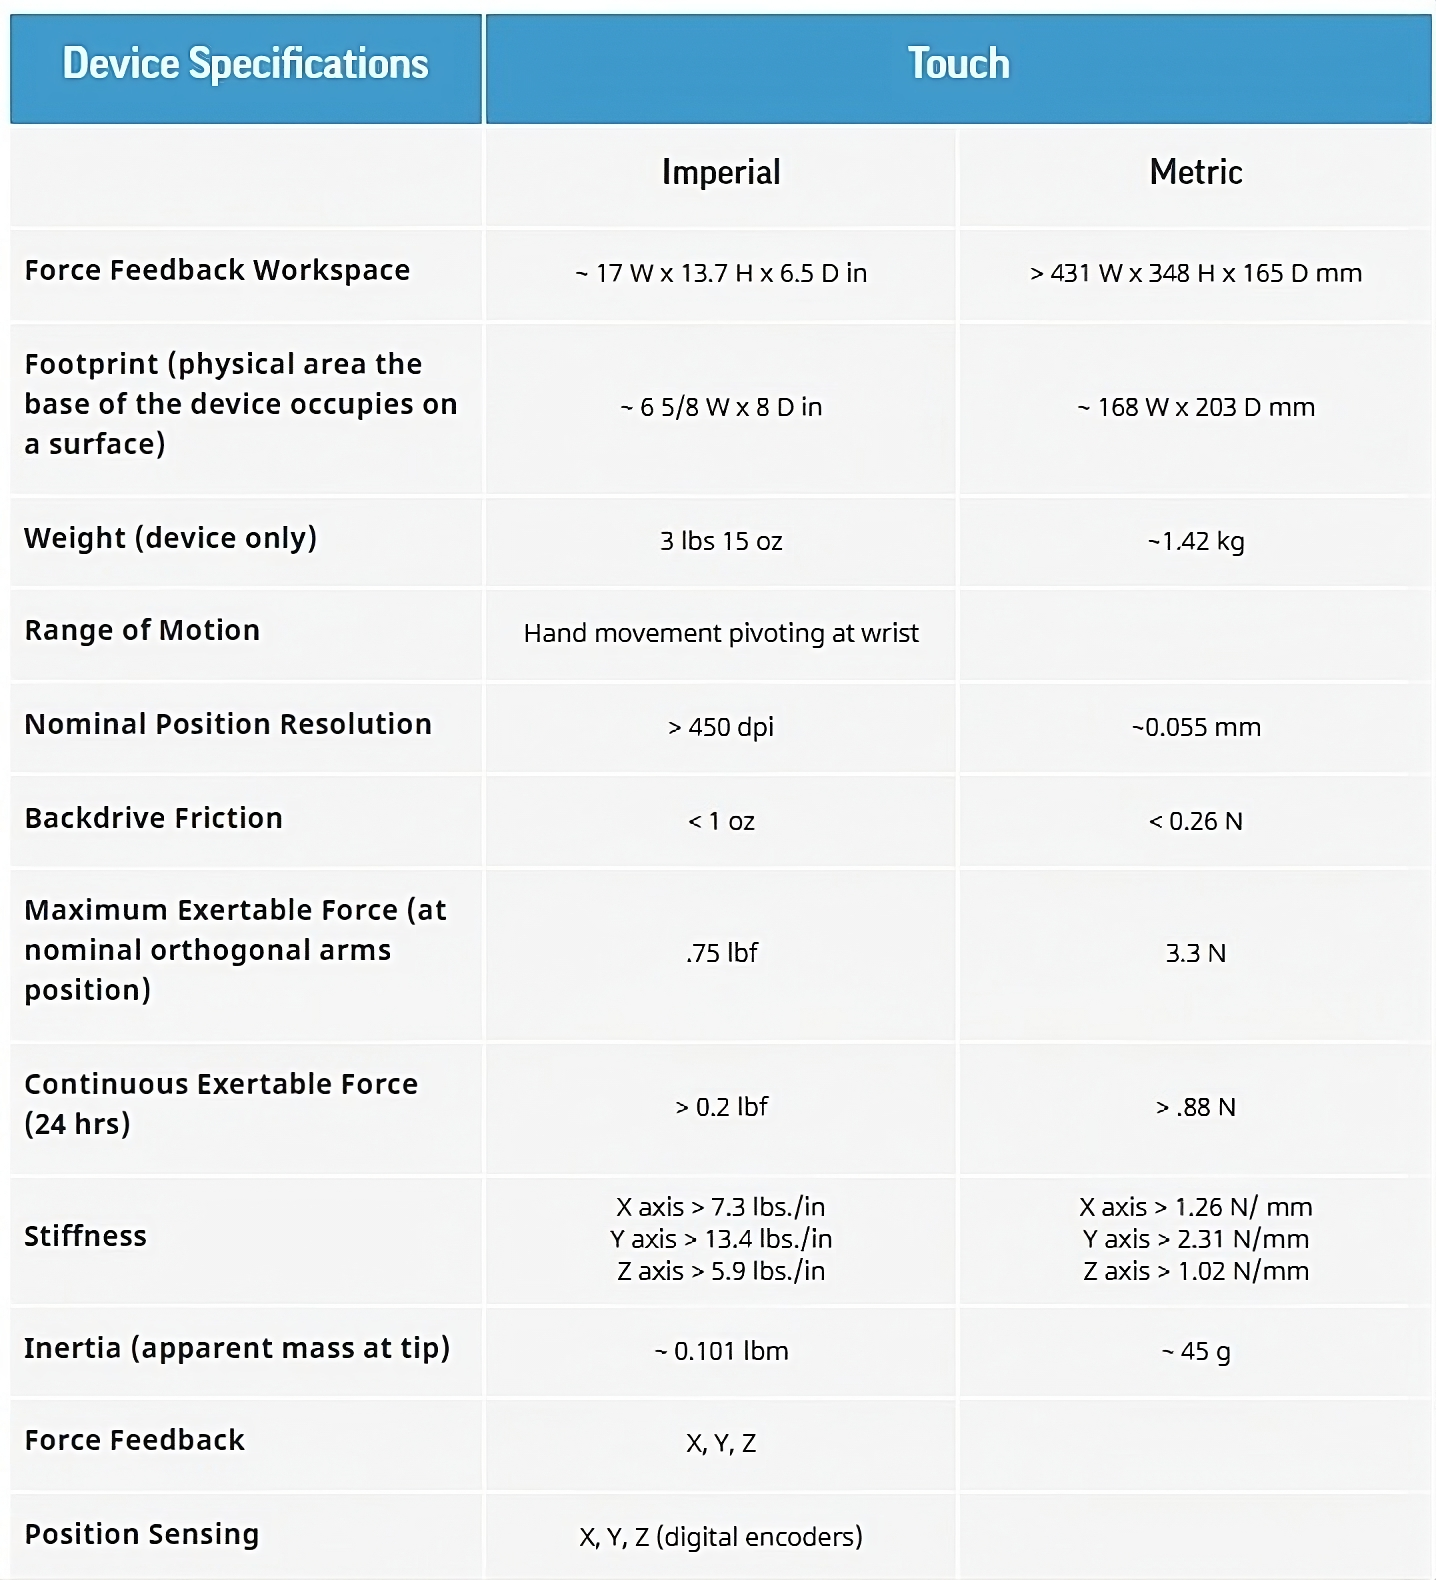
\includegraphics[width=0.75\linewidth]{images/technical_geomagic_touch.png}
    \caption{Especificaciones técnicas del dispositivo háptico Geomagic Touch
        de 3D Systems}
    \label{fig:technical_geomagic_touch}
\end{figure}

\section{Modelo Cinemático del robot serial}

Un robot serial puede representarse como la unión cinemática de distintos
cuerpos rígidos conectados por uniones rotativas o de deslizamiento
\cite{siciliano_robotics_2009}. Para lograr un control óptimo del efector final
del robot, es fundamental comprender cada uno de los elementos presentes en su
análisis cinemático. Esto se debe a que el efector final responderá al
movimiento generado por la acción realizada en cada extremidad del robot.

La cinemática permite expresar este análisis mediante expresiones matemáticas
en función del movimiento de las articulaciones respecto a un punto de
referencia, que generalmente es la base del robot. Este análisis se puede
desglosar en subtemas según su finalidad: la Cinemática Directa, que calcula la
posición y orientación del efector final a partir de los ángulos de rotación de
cada articulación; y la Cinemática Inversa, que determina los ángulos de
rotación en cada articulación necesarios para posicionar el efector final en
coordenadas y orientación deseadas.

\subsection{Matriz de Transformación}

Para poder representar correctamente el movimiento de una articulación del
robot, debemos considerarlo como un cuerpo rígido; es decir, que no presenta
deformación; además que puede ser representado espacialmente por su posición y
orientación\cite{siciliano_robotics_2009}. Es dicha representación la que
podemos definirla bajo un conjunto de transformaciones tanto de rotación como
de traslación.
\begin{figure}[H]
    \centering
    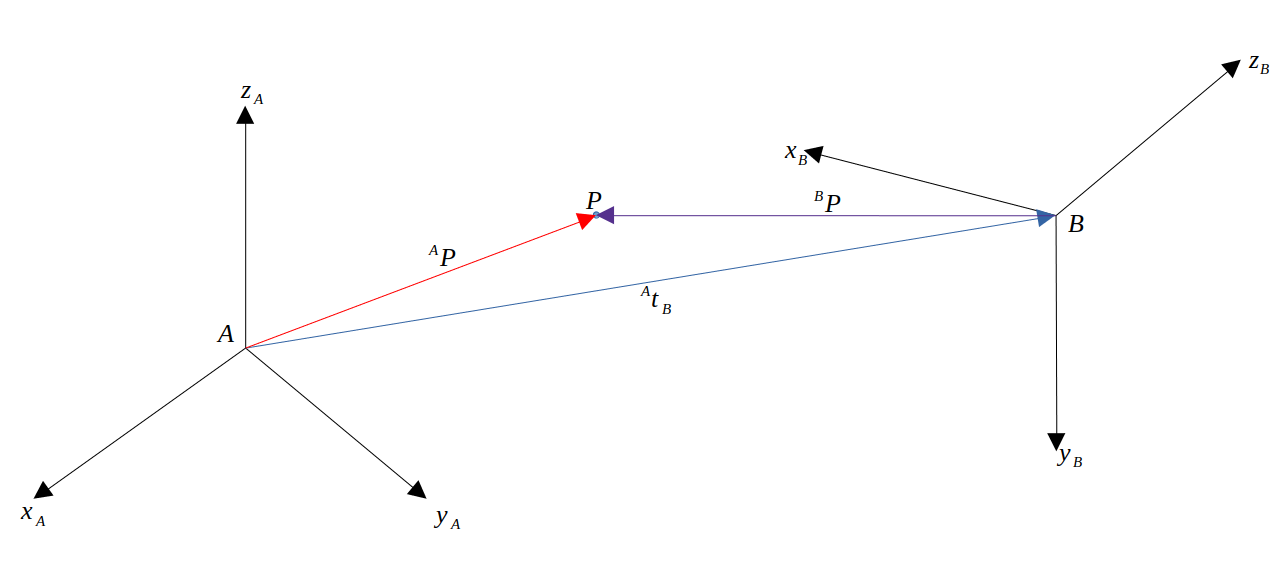
\includegraphics[width=0.95\linewidth]{images/pos_or.png}
    \caption{Posición y orientación de un cuerpo rígido}
    \label{fig:por_or}
\end{figure}

Podemos expresar el punto $\boldsymbol{P}$ en los sistemas de referencia $A$ y
$B$:

$
    \begin{cases}
        ^{A}\boldsymbol{P} = ^{A}x\boldsymbol{\hat{x_A}}  +
        ^{A}y\boldsymbol{\hat{y_A}}+^{A}z\boldsymbol{\hat{z_A}} \\
        ^{B}\boldsymbol{P} = ^{B}x\boldsymbol{\hat{x_B}}  +
        ^{B}y\boldsymbol{\hat{y_B}}+^{B}z\boldsymbol{\hat{z_B}}
    \end{cases}
$

Si proyectamos el punto en $B$ respecto a $A$ podemos realizarlo mediante
la operación vectorial producto punto, lo que resulta en:

$
    \begin{cases}
        ^{A}x = ^{B}\boldsymbol{P} \cdot \boldsymbol{\hat{x_A}} \\
        ^{A}y = ^{B}\boldsymbol{P} \cdot \boldsymbol{\hat{y_A}} \\
        ^{A}z = ^{B}\boldsymbol{P} \cdot \boldsymbol{\hat{z_A}}
    \end{cases}
$

$
    \begin{cases}
        ^{A}x = ^{B}x(\boldsymbol{\hat{x_B}} \cdot \boldsymbol{\hat{x_A}})  +
        ^{B}y(\boldsymbol{\hat{y_B}} \cdot
        \boldsymbol{\hat{x_A}})+^{B}z(\boldsymbol{\hat{z_B}} \cdot
        \boldsymbol{\hat{x_A}}) \\
        ^{A}y = ^{B}x(\boldsymbol{\hat{x_B}} \cdot \boldsymbol{\hat{y_A}})  +
        ^{B}y(\boldsymbol{\hat{y_B}} \cdot
        \boldsymbol{\hat{y_A}})+^{B}z(\boldsymbol{\hat{z_B}} \cdot
        \boldsymbol{\hat{y_A}}) \\
        ^{A}z = ^{B}x(\boldsymbol{\hat{x_B}} \cdot \boldsymbol{\hat{z_A}})  +
        ^{B}y(\boldsymbol{\hat{y_B}} \cdot
        \boldsymbol{\hat{z_A}})+^{B}z(\boldsymbol{\hat{z_B}} \cdot
        \boldsymbol{\hat{z_A}})
    \end{cases}
$

Vectorialmente, podemos expresarlo:
\begin{equation*}
    \begin{bmatrix}
        ^{A}x \\^{A}y\\^{A}z
    \end{bmatrix} =
    \begin{bmatrix}
        \boldsymbol{\hat{x_B}} \cdot \boldsymbol{\hat{x_A}} &
        \boldsymbol{\hat{y_B}} \cdot \boldsymbol{\hat{x_A}} & \boldsymbol{\hat{z_B}}
        \cdot \boldsymbol{\hat{x_A}}                                                 \\
        \boldsymbol{\hat{x_B}} \cdot \boldsymbol{\hat{y_A}} &
        \boldsymbol{\hat{y_B}} \cdot \boldsymbol{\hat{y_A}} & \boldsymbol{\hat{z_B}}
        \cdot \boldsymbol{\hat{y_A}}                                                 \\
        \boldsymbol{\hat{y_B}} \cdot \boldsymbol{\hat{z_A}} &
        \boldsymbol{\hat{y_B}} \cdot \boldsymbol{\hat{z_A}} & \boldsymbol{\hat{z_B}}
        \cdot \boldsymbol{\hat{z_A}}
    \end{bmatrix} \begin{bmatrix}
        ^{B}x \\  ^{B}y \\ ^{B}z
    \end{bmatrix}
\end{equation*}

Operando se consigue la expresión matricial correspondiente a la matriz de
rotación, esta se define como $^{A}\boldsymbol{R}_B$ \cite{siciliano_robotics_2009}. Si
analizamos las rotaciones realizadas en los 3 ejes principales podemos definir
3 matrices elementales de rotación, que son de utilidad al momento de expresar
transformaciones en la orientación.

\begin{equation}
    \boldsymbol{R}_x(\theta) =
    \begin{bmatrix}
        1 & 0            & 0             \\
        0 & \cos{\theta} & -\sin{\theta} \\
        0 & \sin{\theta} & \cos{\theta}
    \end{bmatrix}
    \quad
    \boldsymbol{R}_y(\theta) =
    \begin{bmatrix}
        \cos{\theta}  & 0 & \sin{\theta} \\
        0             & 1 & 0            \\
        -\sin{\theta} & 0 & \cos{\theta}
    \end{bmatrix}
    \quad
    \boldsymbol{R}_z(\theta) =
    \begin{bmatrix}
        \cos{\theta} & -\sin{\theta} & 0 \\
        \sin{\theta} & \cos{\theta}  & 0 \\
        0            & 0             & 1
    \end{bmatrix}
\end{equation}

Para representar una traslación del eje $B$ respecto al eje $A$ veremos que se
puede traducir en una suma vectorial de la posición del sistema $A$ y el vector
$^{A}\boldsymbol{t}_B$

\begin{equation*}
    ^{A}\boldsymbol{P}  = ^{A}\boldsymbol{t}_B +  ^{B}\boldsymbol{P}
\end{equation*}

Si juntamos tanto traslación como rotación obtenemos
\begin{equation*}
    ^{A}\boldsymbol{P}  = ^{A}\boldsymbol{t}_B +  ^{A}\boldsymbol{R}_B \ ^{B}\boldsymbol{P}
\end{equation*}

Matricialmente, podemos reducir la expresión a:
\begin{equation}
    \begin{bmatrix}
        ^{A}\boldsymbol{P} \\1
    \end{bmatrix} = \begin{bmatrix}
        ^{A}\boldsymbol{R}_B & ^{A}\boldsymbol{t}_B \\
        0       & 1
    \end{bmatrix} \begin{bmatrix}
        ^{B}\boldsymbol{P} \\ 1
    \end{bmatrix}
\end{equation}

Entonces la matriz resultante representará la matriz de transformación
homogénea $^{A}\boldsymbol{T}_B$

\subsection{Cinemática Directa}
\begin{figure}[H]
    \centering
    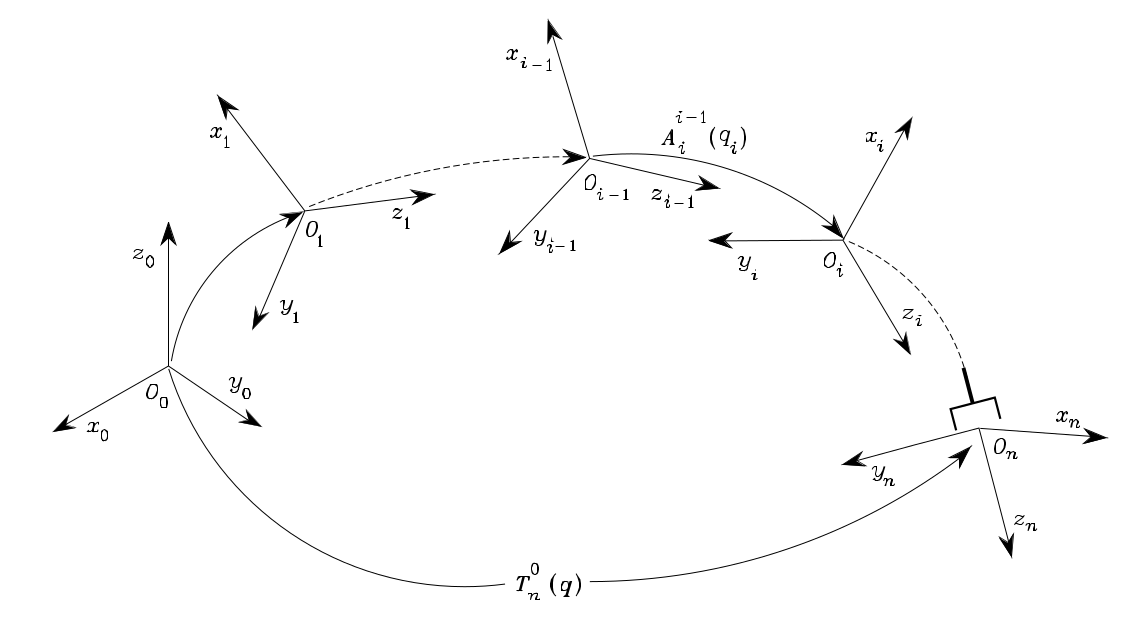
\includegraphics[width=1\linewidth]{images/graf2.png}
    \caption{Transformación de coordenadas en una Cadena cinemática abierta
        \cite{siciliano_robotics_2009}}
    \label{fig:enter-label}
\end{figure}
La Cinemática Directa permite encontrar la posición y orientación del
efector final, tomando como entrada las transformaciones realizadas en cada una
de las extremidades, una después de la otra. Esta cadena de transformaciones
homogéneas se puede expresar como una multiplicación de cada matriz de
transformación aplicada a las extremidades que representa finalmente la matriz
de transformación homogénea general desde la base del robot o sistema de
referencia inercial hasta el efector final.

\begin{equation} \label{t-homog}
    ^{0}\boldsymbol{T}_n = (^{0}\boldsymbol{T}_1)(^{1}\boldsymbol{T}_2)...(^{n-1}\boldsymbol{T}_n)
\end{equation}

El cálculo de la Cinemática Directa no está exento a un solo método; este
dependerá del nivel de complejidad del sistema a representar. Por ejemplo, no
será lo mismo intentar representar un sistema planar de 2 grados de libertad o
tridimensional con 3 grados de libertad, a un sistema con 6 grados de libertad.

\subsubsection{Análisis Geométrico y Trigonométrico}

Este método consiste en usar las relaciones trigonométricas en las formas
geométricas que forman al sistema. Estas permiten expresar la ubicación de
eslabones a través de proyecciones, respecto al eslabón anterior. Es una forma
directa y gráfica de representar las transformaciones de traslación y rotación.
Sin embargo, las expresiones trigonométricas resultantes para sistemas
complejos son poco manejables y, de no ser manejadas correctamente, pueden
inducir al error.

\begin{figure}[H]
    \centering
    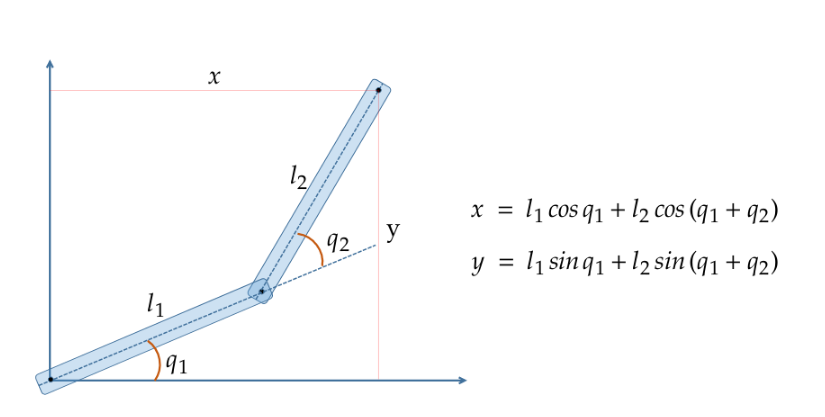
\includegraphics[width=0.75\linewidth]{images/Kinnetics_geom.png}
    \caption{Método geométrico para sistema de 2 grados de libertad}
    \label{fig:placeholder}
\end{figure}

\subsubsection{Método Denavit-Hartenberg}

Este método permite, de manera sistemática, obtener las matrices homogéneas
de cada extremidad mediante un conjunto de pasos tomando en cuenta la
extremidad anterior.
\begin{figure}[H]
    \centering
    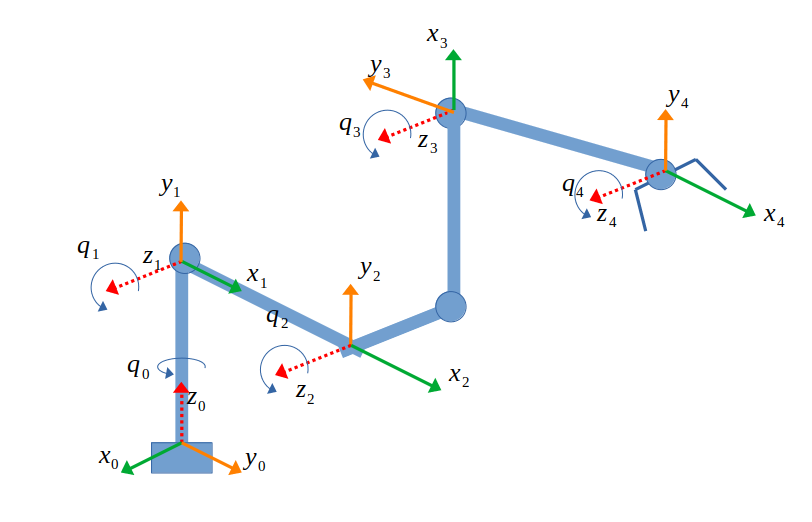
\includegraphics[width=\linewidth]{images/DH_general.png}
    \caption{Método Denavit-Hartenberg}
    \label{fig:enter-label}
\end{figure}

\textbf{Pasos para la elección de los ejes:}
\begin{itemize}
    \item Eje $z_i$: Se ubica $z_i$ sobre el eje de movimiento de la
          articulación siguiente.
    \item El origen de coordenadas se ubica en la intersección de los ejes
          $z_{i-1}$ y $z_i$. Si los ejes son paralelos se ubica en la intersección de
          $z_i$ con la normal en común entre $z_{i-1}$ y $z_i$.
    \item Eje $x_i$: Se ubica en dirección de $z_{i-1}$ x $z_i$. Si los
          ejes son paralelos se ubica en la normal en común entre $z_{i-1}$ y $z_i$.
    \item Eje $y_i$: Se ubica completando el eje coordenado.

\end{itemize}

\textbf{Parámetros a identificar }
\begin{itemize}
    \item $\theta_i$: Rotación del eje $x_{i-1}$ a $x_i$ alrededor del eje
          $z_{i-1}$
    \item $d_i$: Distancia del sistema coordenado $i-1$ a $i$ a lo largo
          del eje $z_{i-1}$ hasta la intersección de $x_i$ con $z_{i-1}$
    \item $a_i$: Distancia de la intersección de $x_i$ con $z_{i-1}$  a lo
          largo del eje $x_{i_1}$ hasta sistema coordenado $i$
    \item $\alpha_i$: Rotación del eje $z_{i-1}$ a $z_i$ alrededor del eje
          $x_{i}$
\end{itemize}

Una vez identificado los parámetros para cada sistema, los ubicamos en un
cuadro:
\\

\begin{table}[H]
    \begin{center}
        \begin{tabular}{| c | c | c | c | c |}
            \hline
            i & $d_i$ & $\theta_i$         & $a_i$ & $\alpha_i$ \\ \hline
            1 & $d_1$ & $\theta_1$ + $q_1$ & $a_1$ & $\alpha_1$ \\ \hline
            2 & $d_2$ & $\theta_2$ + $q_2$ & $a_2$ & $\alpha_2$ \\ \hline
              &       & ...                &       &            \\ \hline
            n & $d_n$ & $\theta_i$ + $q_n$ & $a_n$ & $\alpha_n$ \\ \hline
        \end{tabular}
        \caption{Tabla con parámetros}
        \label{tab:DH}
    \end{center}
\end{table}

Para llevar los parámetros a una Transformación homogénea se toma este
orden de para cada movimiento realizado:
\begin{enumerate}
    \item Rotación $\theta_i$ en el eje $z_{i-1}$
    \item Traslación $d_i$ en el eje $z_{i-1}$
    \item Traslación $a_i$ en el eje $x_{i}$
    \item Rotación $\alpha_i$ en el eje $z_{i}$
\end{enumerate}
Multiplicando cada matriz homogénea se consigue:

\begin{equation*}
    ^{i-1}\boldsymbol{T}_{i}(\theta_i,d_i,a_i,\alpha_i)=
    \begin{bmatrix}
        \cos{\theta_i} & -\cos{\alpha_i}\sin{\theta_i}
                       & \sin{\alpha_i}\sin{\theta_i}  & a_i\cos{\theta_i}       \\
        \sin{\theta_i} & \cos{\alpha_i}\cos{\theta_i}
                       & -\sin{\alpha_i}\cos{\theta_i} & a_i\sin{\theta_i}       \\
        0              & \sin{\alpha_i}                & \cos{\alpha_i}    & d_i \\
        0              & 0                             & 0                 & 1
    \end{bmatrix}
\end{equation*}

La ecuación \ref{t-homog} permite obtener la representación de la posición
y orientación del efector final respecto a la base del robot.

\subsection{Matriz Jacobiana}

Para poder expresar la velocidad lineal y angular del efector final en
función de la velocidad rotacional de cada articulación se define la matriz
Jacobiana.

\begin{equation}
    \boldsymbol{v} = \boldsymbol{J}\boldsymbol{\dot{q}}
    \label{Jacobian_relation}
\end{equation}

Esta matriz relaciona de forma lineal las velocidades articulares con las
velocidades en el espacio de trabajo del efector final mediante las
contribuciones realizadas por cada articulación. Esta matriz se denomina
Jacobiano Geométrico

\begin{equation}
    \begin{cases}
        \boldsymbol{\dot{p}_e} =
        \boldsymbol{J_P}(\boldsymbol{q})\boldsymbol{\dot{q}} \\
        \boldsymbol{{\omega}_e} =
        \boldsymbol{J_O}(\boldsymbol{q})\boldsymbol{\dot{q}}
    \end{cases}
\end{equation}

\begin{equation}
    \boldsymbol{J_G} = \begin{bmatrix}
        \boldsymbol{J_P} \ \ 0 \\
        0 \ \ \boldsymbol{J_O}
    \end{bmatrix}
\end{equation}

Conociendo la ecuación que representa la cinemática directa del robot con el
que se trabajará se puede obtener una expresión analítica que relaciona la
derivada de la traslación y rotación del efector final respecto al origen del
sistema inercial del robot:

\begin{equation}
    \boldsymbol{J_A} = \frac{\partial f(\boldsymbol{q})}{\partial
        \boldsymbol{q}}
\end{equation}

\subsection{Cinemática Inversa}

La Cinemática Inversa permite calcular las configuraciones articulares de
cada elemento en la cadena de articulaciones necesario para lograr una posición
y orientación deseada.
El cálculo de la cinemática inversa en robots como el UR5 de 6 grados de
libertad resulta tedioso bajo la directriz de métodos de resolución de
ecuaciones clásicos, puesto que se encuentran con expresiones no lineales
incompatibles a la resolución por sistema de ecuaciones. Por otro lado, existe
el método numérico; este forma de resolución es de naturaleza recursiva y hace
uso de técnicas como la minimización de una función costo del error respecto a
la posición actual y la posición deseada del efector final.

% Las soluciones por métodos numéricos propuestos son la resolución por Método de Gradiente, donde se toma una función costo dependiente de los valores articulares del robot, cuya gradiente permitirá encontrar valores para cada articulación acercando la posición del efector final a la posición deseada; y, por otro lado, el Método de Optimización Cuadrática, donde se plantea un problema de minimización con la función costo definida anteriormente.

\subsubsection{Método Gradiente}
De la cinemática directa:
\begin{equation*}
    \boldsymbol{x}_d = f(\boldsymbol{q}) \longrightarrow \boldsymbol{x}_d -
    f(\boldsymbol{q}) = 0
\end{equation*}
Donde la expresión resultante es el error respecto a la posición deseada.
Con esta expresión podemos definir la función costo $g(\boldsymbol{q})$
\begin{equation*}
    g(\boldsymbol{q}) = \frac{1}{2} \|\boldsymbol{x}_d -
    f(\boldsymbol{q})\|^2
\end{equation*}

Se calcula el gradiente de $g(\boldsymbol{q})$:
\begin{equation*}
    \nabla g(\boldsymbol{q}) = -(\frac{\partial f(\boldsymbol{q})}{\partial
        \boldsymbol{q}})^T (\boldsymbol{x}_d - f(\boldsymbol{q}))
\end{equation*}

Finalmente, se puede aplicar el método gradiente de manera recursiva
mediante un parámetro $\alpha$ que determinará el tamaño de paso en el avance
del gradiente hasta encontrar los valores articulares adecuados.
\begin{equation}
    \boldsymbol{q}_{k+1} = \boldsymbol{q}_k + \alpha\boldsymbol{J}^T
    (\boldsymbol{q}_k)(\boldsymbol{x}_d-f(\boldsymbol{q}_k))
\end{equation}

\subsubsection{Método por Optimización Cuadrática}
Partiendo de la función costo $g(\boldsymbol{q})$ se define un problema de
minimización, con $\boldsymbol{e}$ como el error de posición, de la forma:
\begin{mini*}|s|[0]
    {\boldsymbol{\dot{q}}}{\|\boldsymbol{J(q)}\boldsymbol{\dot{q}} -
    \boldsymbol{e}\|^2}
    {}
    {\label{eq:minimizationProblem1}}
\end{mini*}

Expandiendo y ordenando podemos plantear un problema cuadrático de la
forma:
\begin{mini}|s|[0]
    {\boldsymbol{\dot{q}}}{\frac{1}{2}\boldsymbol{\dot{q}}^{T}\boldsymbol{H}\boldsymbol{\dot{q}}
    + {\nabla g(\boldsymbol{q})}^T\boldsymbol{\dot{q}}}
    {}
    {\label{eq:minimizationProblem}}
\end{mini}
donde $\boldsymbol{H} =\boldsymbol{J(q)}^{T}\boldsymbol{J(q)} $, como
matriz Hesiana y el gradiente $\nabla g(\boldsymbol{q}) =
    -(\boldsymbol{J(q)}^{T}\boldsymbol{e})$

% \\

% $\boldsymbol{q}$ : configuración articular \\
% $\boldsymbol{\dot{q}}$: velocidad articular \\
% $\boldsymbol{J(q)}$ : Matriz Jacobiana \\
% $\boldsymbol{e}$ : error de posición \\
% $\boldsymbol{H}$ : Matriz Hesiana\\
% $\nabla g(\boldsymbol{q})$ : Gradiente

\section{Modelo Dinámico del robot serial }

El modelo dinámico permite relacionar el movimiento del robot mediante el
análisis de la fuerza y torques aplicados en cada articulación. Mediante este
análisis se pueden determinar con mayor fiabilidad un sistema de simulación del
robot y el modelamiento de un sistema de control adecuado para entornos reales.
Sin embargo, encontrar el modelo dinámico de un robot manipulador implica poder
determinar variables matriciales que gobiernan el comportamiento del robot,
como la matriz de inercia. Ante este problema, existen métodos matemáticos para
el diseño de modelos dinámicos, sea de manera analítica, mediante ecuaciones
simbólicas; o de manera numérica, mediante recursividad.

\subsection{Newton Euler}
Este método es de naturaleza recursiva, puesto que los valores se operarán
con los obtenidos anteriormente. Es esta naturaleza la que permite obtener la
dinámica inversa, donde se consiguen las fuerzas y torques necesarios para
lograr un movimiento deseado. Además, permite establecer un algoritmo que,
sumado a herramientas computacionales, logra realizar el cálculo con mayor
rapidez.

El método Newton-Euler realiza un análisis desde la formulación de la
$2^{da}$ ley de Newton para traslación y la $2^{da}$ ley de Euler para la
rotación.
\begin{equation*}
    \boldsymbol{f}_i = \boldsymbol{f}_{i+1} +
    m_i\ddot{\boldsymbol{p}}_{c_i}-m_i\boldsymbol{g}_0
\end{equation*}
\begin{equation*}
    \boldsymbol{\mu}_i = \boldsymbol{\mu}_{i+1} -
    \boldsymbol{f}_{i}\times\boldsymbol{r_{i-1,c_i}}+\boldsymbol{f}_{i+1}\times\boldsymbol{r_{i,c_i}}+\boldsymbol{I}_i\times\dot{\boldsymbol{\omega}}_i+\boldsymbol{\omega}_i\times\boldsymbol{I}_i\boldsymbol{\omega}_i
\end{equation*}

Para un eslabón $i$ con matriz de rotación $^iR_{i-1}$ podemos obtener
\cite{fundamentos_robo}:

\textbf{Velocidad Angular }
\begin{equation*}
    \boldsymbol{\omega}_i = \begin{cases}
        ^{i}\boldsymbol{R}_{i-1} (\boldsymbol{\omega}_{i-1} +
        \dot{q_i}\boldsymbol{z}_{i-1}) & \text{, si es de rotación} \\
        ^{i}\boldsymbol{R}_{i-1} (\boldsymbol{\omega}_{i-1}) & \text{, si es
            de prismático}
    \end{cases}
\end{equation*}

\textbf{Aceleración Angular }
\begin{equation*}
    \dot{\boldsymbol{\omega}_i} = \begin{cases}
        ^{i}\boldsymbol{R}_{i-1} (\dot{\boldsymbol{\omega}}_{i-1} +
        \ddot{q_i}\boldsymbol{z}_{i-1} +
        \dot{q_i}\boldsymbol{w}_{i-1}\times\boldsymbol{z}_{i-1}) & \text{, si
            es de rotación} \\
        ^{i}\boldsymbol{R}_{i-1} (\dot{\boldsymbol{\omega}}_{i-1}) & \text{, si
            es de prismático}
    \end{cases}
\end{equation*}

\textbf{Aceleración Lineal}
\begin{equation*}
    \ddot{\boldsymbol{p}}_i =
    ^{i}\boldsymbol{R}_{i-1}\ddot{\boldsymbol{p}}_{i-1} +
    \dot{\boldsymbol{\omega}}_i\times\boldsymbol{r}_{i-1,i}+\boldsymbol{\omega}_i\times(\boldsymbol{\omega}_i\times\boldsymbol{r}_{i-1,i})
\end{equation*}

\textbf{Aceleración del centro de masa}
\begin{equation*}
    \ddot{\boldsymbol{p}}_{c_i} = \ddot{\boldsymbol{p}}_{i} +
    \dot{\boldsymbol{\omega}}_i\times\boldsymbol{r}_{i,c_i}+\boldsymbol{\omega}_i\times(\boldsymbol{\omega}_i\times\boldsymbol{r}_{i,c_i})
\end{equation*}

Para calcular estos valores adecuadamente se toma como valores
iniciales\cite{fundamentos_robo}:

$\boldsymbol{\omega}_0 = \begin{bmatrix}
        0 \\0\\0
    \end{bmatrix}$ \ \ \ , $\dot{\boldsymbol{\omega}}_0 = \begin{bmatrix}
        0 \\0\\0
    \end{bmatrix}$ \ \ \, $\dot{\boldsymbol{p}} =\begin{bmatrix}
        0 \\0\\0
    \end{bmatrix} - \boldsymbol{g}$ \ \ \ , $\boldsymbol{z}_0 =
    \boldsymbol{z}_1 = ...= \boldsymbol{z}_n  = \begin{bmatrix}
        0 \\0\\1
    \end{bmatrix}$

El cálculo de la fuerza y de torques implicará un cálculo recursivo
inverso, es decir, se tomará el valor actual para calcular el anterior.
\begin{equation}
    \begin{cases}
        \boldsymbol{f}_i = ^{i}\boldsymbol{R}_{i+1} \boldsymbol{f}_{i+1} +
        m_i\boldsymbol{\ddot{p}}_{c_i} \\
        \boldsymbol{\mu}_i = ^{i}\boldsymbol{R}_{i+1}
        \boldsymbol{\mu}_{i+1} -
        \boldsymbol{f}_{i}\times(\boldsymbol{r}_{i-1,i}+\boldsymbol{r}_{i,c_i}) +
        ^{i}\boldsymbol{R}_{i+1}\boldsymbol{f}_{i+1}\times\boldsymbol{r}_{i,c_i} +
        \boldsymbol{I}_i\dot{\boldsymbol{\omega}}_i +
        {\boldsymbol{\omega}}_i\times\boldsymbol{I}_i\boldsymbol{\omega}_i
    \end{cases}
\end{equation}

De manera similar a las velocidades y aceleraciones, los valores iniciales
estarán expresados por:

$\boldsymbol{\mu}_{N+1} = \begin{bmatrix}
        0 \\0\\0
    \end{bmatrix}$ \ \ \ $\boldsymbol{f}_{N+1} = \begin{bmatrix}
        0 \\0\\0
    \end{bmatrix}$\ \ \ $^N\boldsymbol{R}_{N+1} = \begin{bmatrix}
        1 & 0 & 0 \\0&1&0\\0&0&1
    \end{bmatrix}$

Con las expresiones y términos calculados, podemos definir los torques o
fuerzas generalizados del modelo dinámico y por consiguiente, el modelo
dinámico:

\begin{equation}
    \begin{cases}
        \boldsymbol{\tau}_i = {\boldsymbol{\mu}_i}^T
        {^{i}\boldsymbol{R}_{i-1}} \boldsymbol{z}_{i-1} \\
        \boldsymbol{\tau}_i = {\boldsymbol{f}_i}^T
        {^{i}\boldsymbol{R}_{i-1}} \boldsymbol{z}_{i-1}
    \end{cases}
    \label{eq:EcuacionDinamica}
\end{equation}

Reordenando podemos obtener la ecuación dinámica en el espacio articular
para un robot:

\begin{equation}
    \boldsymbol{u} =
    \boldsymbol{M}(\boldsymbol{q})\cdot\boldsymbol{\ddot{q}}+\boldsymbol{B}(\boldsymbol{q},\boldsymbol{\dot{q}})\cdot\boldsymbol{\dot{q}}+\boldsymbol{G}(\boldsymbol{q})
\end{equation}

Para poder trabajar con el seguimiento a trayectorias se necesita cambiar
el espacio de trabajo a uno operacional. Usando la relación de velocidades
\ref{Jacobian_relation} podemos reformular la ecuación dinámica de la forma:

\begin{equation}
    \boldsymbol{F} = \boldsymbol{M_x}(\boldsymbol{q})\boldsymbol{\ddot{x}} + \boldsymbol{\mu}(\boldsymbol{q}, \boldsymbol{\dot{q}}) + \boldsymbol{\rho}(\boldsymbol{q})
    \label{eq:dinamica_operacional}
\end{equation}

Donde $\boldsymbol{M_x}(\boldsymbol{q})$ es la matriz de inercia operacional:

\begin{equation}
    \boldsymbol{M_x}(\boldsymbol{q}) = \left( \boldsymbol{J}(\boldsymbol{q}) \boldsymbol{M}^{-1}(\boldsymbol{q}) \boldsymbol{J}^T(\boldsymbol{q}) \right)^{-1}
\end{equation}

mientras que $\boldsymbol{\mu}(\boldsymbol{q}, \boldsymbol{\dot{q}})$ y $\boldsymbol{\rho}(\boldsymbol{q})$ son, respectivamente, las
proyecciones de los efectos de Coriolis/centrípetos y de gravedad al espacio
operacional (pendiente de detallar su expresión explícita).

\section{Control por Dinámica Inversa}
\subsection{Espacio Articular}
El problema se centra en encontrar los valores de torque necesarios en cada
articulación para que el efector final del robot alcance una posición y
velocidad articular deseada. Se parte de la ecuación dinámica del robot, el
cual podemos calcular con la ecuación \ref{eq:EcuacionDinamica} usando el
método de Newton Euler. Una vez obtenida se ordena de forma que se expresa de
la forma:

\begin{equation}
    \boldsymbol{\tau(q,\dot{q},\ddot{q})} = \boldsymbol{M(q)\cdot \ddot{q}} +
    \boldsymbol{C(q,\dot{q}) \cdot \dot{q}} + \boldsymbol{G(q)}
\end{equation}

Definimos:
\begin{equation*}
    \boldsymbol{u}=\boldsymbol{\tau(q,\dot{q},\ddot{q})}
\end{equation*}
\begin{equation*}
    \boldsymbol{n(q,\dot{q})}=\boldsymbol{C(q,\dot{q}) \cdot \dot{q}} +
    \boldsymbol{G(q)}
\end{equation*}

Reordenamos:
\begin{equation}
    \boldsymbol{M(q)\ddot{q}} + \boldsymbol{n(q,\dot{q})} = \boldsymbol{u}
    \label{eq:EcuacionDinamica_1}
\end{equation}

Donde $\boldsymbol{M(q)}$ representa la matriz de Inercia,
$\boldsymbol{n(q,\dot{q})}$ representa las no linealidades del sistema (Efecto
Coriolis y Gravedad) y $\boldsymbol{u}$ será el vector de control a encontrar
en función del sistema que permita linealizar la dinámica del sistema.
Al ser $\boldsymbol{M(q)}$ de rango completo podemos reordenar la ecuación
\ref{eq:EcuacionDinamica_1} en función de $\boldsymbol{u}$ y observar que es un
sistema lineal \cite{siciliano_robotics_2009}. Así podemos definir una
expresión que contrarreste los torques generados por las no linealidades de la
forma:

\begin{equation}
    \boldsymbol{u} = \boldsymbol{M(q)y} + \boldsymbol{n(q,\dot{q})}
    \label{eq:EcuacionDinamica_2}
\end{equation}

Donde $\boldsymbol{y}$ es una aceleración de referencia aún por determinar.

Reemplazando \ref{eq:EcuacionDinamica_2} en \ref{eq:EcuacionDinamica_1} se
obtiene:

\begin{equation}
    \boldsymbol{\ddot{q}} = \boldsymbol{y}
    \label{relacion_dinamica}
\end{equation}

De esta manera se puede denominar al sistema encontrado como lineal y
desacoplado respecto a $\boldsymbol{y}$ puesto que cada componente de este
afectará individualmente a su componente de aceleración articular respectivo.
Así el problema queda simplificado a hallar el vector $\boldsymbol{y}$, ahora
denominada ley de control.

Podemos definir una ley de control de la forma:
\begin{equation}
    \boldsymbol{y}=-\boldsymbol{K_P\cdot{q}}-\boldsymbol{K_D\cdot{\dot{q}}}+\boldsymbol{r}
\end{equation}

Donde $\boldsymbol{r}$ será el componente de referencia usado para el
seguimiento a la trayectoria.

Usando \ref{relacion_dinamica} podemos definir su equivalente como ecuación de
segundo orden:

\begin{equation}
    \boldsymbol{\ddot{q}}+\boldsymbol{K_P\cdot{q}}+\boldsymbol{K_D\cdot{\dot{q}}}=\boldsymbol{r}
    \label{ley_1}
\end{equation}

Para que el sistema siga una trayectoria deseada se define $\boldsymbol{r}$ de
forma que incluya la aceleración deseada $\boldsymbol{\ddot{q_d}}$ y los
términos que permitan dirigir el sistema a la posición y velocidad articular
deseada.

\begin{equation}
    \boldsymbol{r}=
    \boldsymbol{\ddot{q_d}}+\boldsymbol{K_P\cdot{q_d}}+\boldsymbol{K_D\cdot{\dot{q_d}}}
    \label{ley_2}
\end{equation}

Sustituyendo \ref{ley_2} en \ref{ley_1} y definiendo $\boldsymbol{e} =
    \boldsymbol{q_d-q}$ obtenemos:

\begin{equation}
    \boldsymbol{\ddot{e}}+\boldsymbol{K_D\cdot{\dot{e}}}+\boldsymbol{K_P\cdot{e}}=0
    \label{error_din}
\end{equation}

Esta ecuación representa la dinámica del error de posición en una trayectoria
deseada, permitiendo llevar el error de seguimiento a 0 eligiendo las matrices
de ganancias $\boldsymbol{K_P}$ y $\boldsymbol{K_D}$ adecuadas. Así finalmente
podemos definir la ley de control para un control por dinámica inversa
despejando $\boldsymbol{\ddot{q}}$ de la ecuación \ref{error_din} y
sustituyendo en la ecuación dinámica del sistema \ref{eq:EcuacionDinamica_1}.

\begin{equation}
    \boldsymbol{u} =
    \boldsymbol{M(q)}[\boldsymbol{\ddot{q_d}}+\boldsymbol{K_D}(\boldsymbol{\dot{q_d}}-\boldsymbol{\dot{q}})+\boldsymbol{K_P}(\boldsymbol{{q_d}}-\boldsymbol{{q}})]+\boldsymbol{n(q,\dot{q})}
\end{equation}

\subsection{Espacio Operacional}
Trabajar en el espacio operacional consiste en encontrar el esfuerzo de control
necesario para llevar al efector final del robot a una posición cartesiana
deseada $\boldsymbol{x}_d$. Para hallar el vector que representará nuestra ley de control
partiremos de la expresión \ref{Jacobian_relation}, considerando $\boldsymbol{J}=\boldsymbol{J_A}$, que
permite relacionar la velocidad en el espacio articular con el espacio
operacional.

\begin{equation}
    \dot{\boldsymbol{x}}  = \boldsymbol{v} = \boldsymbol{J\dot{q}}
\end{equation}

\begin{equation}
    \boldsymbol{\ddot{x}} = \boldsymbol{J(q)\cdot\ddot{q}} +
    \dot{\boldsymbol{J}}(\boldsymbol{q,\dot{q}})\cdot\dot{\boldsymbol{q} }
\end{equation}

De lo definido en la dinámica articular volvemos a definir un sistema
desacoplado para un vector de entrada $\boldsymbol{y}$, por lo que el sistema vuelve a ser
simplificado a la búsqueda de una ley de control que permita el seguimiento a
la trayectoria, pero esta vez en el espacio operacional.

Se define la ley de control:
\begin{equation}
    \boldsymbol{y} =
    \boldsymbol{J}^{-1}(\boldsymbol{q})\cdot(\boldsymbol{\ddot{x}}_d +
    \boldsymbol{K_D}\cdot\dot{\boldsymbol{e}} + \boldsymbol{K_P}\cdot
    \boldsymbol{e} -
    \dot{\boldsymbol{J}}(\boldsymbol{q,\dot{q}})\cdot\dot{\boldsymbol{q} })
\end{equation}

\section{Control por Modo Deslizante}

\subsection{Introducción al control por modo deslizante (SMC)}
El control por modo deslizante (SMC, por sus siglas en inglés) es un enfoque de
control no lineal diseñado para dirigir el comportamiento de un sistema hacia
un régimen dinámico específico, definido a través de una superficie de
deslizamiento. El objetivo es que el sistema "deslice" sobre esta superficie,
logrando así que la trayectoria del sistema se mantenga cerca de la deseada a
pesar de perturbaciones y no linealidades. Aunque una de las desventajas de
este método es el fenómeno de chattering, pequeñas oscilaciones indeseadas en
la ley de control, el SMC es especialmente robusto y resistente a variaciones
en el sistema y pequeñas perturbaciones. Esto lo convierte en una opción
valiosa para aplicaciones en entornos inciertos o dinámicos, como es el caso de
la cirugía robótica.

Este método tiene ventajas significativas para el control de sistemas robóticos
en contextos donde existen incertidumbres y no linealidades, como en
aplicaciones quirúrgicas para sutura. Su robustez permite mantener un
rendimiento adecuado a pesar de variaciones inesperadas en el entorno, como el
comportamiento dinámico de los tejidos. Además, el SMC es eficaz en el manejo
de dinámicas no lineales, facilitando la adaptación a cambios sin necesidad de
un modelo preciso del sistema. Su implementación es también relativamente
sencilla, ya que se basa en el diseño de superficies de deslizamiento,
reduciendo la complejidad matemática requerida en comparación con otros
métodos. La flexibilidad en la definición de estas superficies permite adaptar
el control a los requisitos específicos de cada tarea, optimizando así el
desempeño de los manipuladores robóticos UR5 en entornos quirúrgicos
\cite{utkin_sliding_mode_control}.

\subsection{Diseño del control SMC}

El \textbf{control por modo deslizante} (Sliding Mode Control, SMC) es una
técnica robusta ampliamente utilizada para sistemas no lineales. Su objetivo
principal es forzar al sistema a seguir una superficie de deslizamiento, donde
la dinámica se vuelve robusta frente a perturbaciones y modelos inexactos. Para
ello, se diseña una ley de control que garantice que la trayectoria del sistema
converja hacia dicha superficie y permanezca en ella.

Primero se define una función de Lyapunov adecuada para garantizar estabilidad.
En este caso, se emplea una función cuadrática:

\[
    V(x) = \frac{1}{2} s^2
\]

donde la función de deslizamiento está dada por:

\[
    s(x) = \dot{e} + \lambda e
\]

Aquí, \( e = x - x_d \) es el error entre el estado actual \( x \) y el deseado
\( x_d \), y \( \lambda \) es una constante positiva que ajusta la
convergencia.

Para asegurar estabilidad, deben cumplirse tres condiciones fundamentales:

\begin{itemize}
    \item \( V(x) > 0 \) para todo \( x \neq x_d \) (positividad).
    \item \( \dot{V}(x) < 0 \), lo que implica convergencia hacia la superficie
          de deslizamiento.
    \item El sistema debe alcanzar la superficie en tiempo finito y luego
          deslizarse sobre ella.
\end{itemize}

La derivada de Lyapunov es:

\[
    \dot{V} = s \dot{s} = s(\ddot{e} + \lambda \dot{e})
\]

A partir del modelo dinámico del manipulador:

\[
    \boldsymbol{\tau} = \boldsymbol{M} \cdot \boldsymbol{\ddot{q}} + \boldsymbol{C} \cdot \boldsymbol{\dot{q}} + \boldsymbol{G}
\]

se proyecta al espacio cartesiano mediante el Jacobiano \( \boldsymbol{J}_a \), obteniendo:

\[
    \boldsymbol{\ddot{x}} = \boldsymbol{J}_a \cdot \boldsymbol{M}^{-1} \cdot (\boldsymbol{\tau} - \boldsymbol{C} \cdot \boldsymbol{\dot{q}} - \boldsymbol{G}) + \boldsymbol{\dot{J}}_a
    \cdot \boldsymbol{\dot{q}} \tag{1}
\]

La superficie de deslizamiento en el espacio cartesiano se define como:

\[
    \boldsymbol{S} = \boldsymbol{\dot{x}} - \boldsymbol{\dot{x}}_{\text{des}} + \lambda (\boldsymbol{x} - \boldsymbol{x}_{\text{des}})
\]

y su derivada:

\[
    \boldsymbol{\dot{S}} = \boldsymbol{\ddot{x}} - \boldsymbol{\ddot{x}}_{\text{des}} + \lambda (\boldsymbol{\dot{x}} -
    \boldsymbol{\dot{x}}_{\text{des}})
\]

La ley de control se diseña para que:

\[
    \boldsymbol{\dot{S}} = -k \cdot \boldsymbol{S} - k_2 \cdot \tanh(k_3 \cdot \boldsymbol{S})
\]

con ganancias positivas \( k, k_2, k_3 \); en la implementación sobre el
manipulador, $k$ y $k_2$ se aplican como vectores diagonales (una ganancia por
eje cartesiano), mientras que $k_3$ se mantiene como una única ganancia
escalar. Esto garantiza que \( \dot{V} = \boldsymbol{S}^T
\boldsymbol{\dot{S}} < 0 \), cumpliendo la condición de estabilidad.

Sustituyendo la ecuación \((1)\) en la expresión de \( \boldsymbol{\dot{S}} \), se obtiene
la ecuación final para el torque de control:

\[
    \boldsymbol{\tau} = \boldsymbol{M} \cdot \boldsymbol{J}_a^{-1} \cdot \left[ -k \cdot \boldsymbol{S} - k_2 \cdot \tanh(k_3 \cdot \boldsymbol{S})
        - \left( \boldsymbol{\dot{J}}_a \cdot \boldsymbol{\dot{q}} - \boldsymbol{\ddot{x}}_{\text{des}} + \lambda (\boldsymbol{\dot{x}} -
        \boldsymbol{\dot{x}}_{\text{des}}) \right) \right] + \boldsymbol{C} \cdot \boldsymbol{\dot{q}} + \boldsymbol{G}
\]

Esta ley de control garantiza el seguimiento deseado incluso en presencia de
perturbaciones, aprovechando la robustez inherente del enfoque SMC.

\begin{itemize}
    \item \textbf{\( \boldsymbol{\tau} \)}: Torque aplicado al sistema.
    \item \textbf{\( \boldsymbol{M} \)}: Matriz de masa (o inercia).
    \item \textbf{\( \boldsymbol{\ddot{q}} \)}: Aceleración generalizada.
    \item \textbf{\( \boldsymbol{\dot{q}} \)}: Velocidad generalizada.
    \item \textbf{\( \boldsymbol{q} \)}: Posición articular.
    \item \textbf{\( \boldsymbol{C} \)}: Matriz de Coriolis y centrífuga.
    \item \textbf{\( \boldsymbol{G} \)}: Vector de fuerzas de gravedad.
    \item \textbf{\( \boldsymbol{J}_a \)}: Jacobiano de la configuración.
    \item \textbf{\( \boldsymbol{\dot{J}}_a \)}: Derivada temporal del Jacobiano.
    \item \textbf{\( \boldsymbol{x} \)}: Posición en el espacio cartesiano.
    \item \textbf{\( \boldsymbol{\dot{x}} \)}: Velocidad cartesiana.
    \item \textbf{\( \boldsymbol{\ddot{x}} \)}: Aceleración cartesiana.
    \item \textbf{\( \boldsymbol{x}_{\text{des}} \)}, \( \boldsymbol{\dot{x}}_{\text{des}} \), \(
          \boldsymbol{\ddot{x}}_{\text{des}} \): Referencias deseadas.
    \item \textbf{\( \lambda \)}: Ganancia de la superficie de deslizamiento.
    \item \textbf{\( \boldsymbol{S} \)}: Función de deslizamiento.
    \item \textbf{\( \boldsymbol{\dot{S}} \)}: Derivada de la función de deslizamiento.
    \item \textbf{\( k \)}, \textbf{\( k_2 \)}, \textbf{\( k_3 \)}: Ganancias
          del controlador.
    \item \textbf{\( \tanh \)}: Función tangente hiperbólica, usada para
          suavizar el control discontinuo.
    \item \textbf{\( \# \)}: Símbolo que representa la pseudoinversa (si
          aplica).
\end{itemize}

\section{Control por Impedancia}

% Uno de los modelos de control enfocados en la interacción con el entorno es el Control por Impedancia. Esta arquitecura de control está enfocada en reaccionar a fuerzas externas aplicadas en el efector final. Su ley de control interpreta al error en el espacio operacional como un sistema masa resorte amortiguado, donde el objetivo.

El control dinámico por impedancia es un enfoque diseñado para regular el
comportamiento del manipulador durante la interacción física con su entorno,
definiendo una relación dinámica específica entre las fuerzas de contacto y el
error de posición. El objetivo es que el sistema emule el comportamiento de un
mecanismo virtual de masa-resorte-amortiguador, logrando así que el robot
``ceda'' o aplique fuerza de manera controlada de acuerdo con los requisitos de
la tarea, a pesar de las restricciones del entorno. Aunque una de las
principales dificultades de este método es la necesidad de un modelo dinámico
preciso o la inclusión de sensores de fuerza/torque para evitar comportamientos
imprevistos, el control por impedancia es especialmente adecuado para
garantizar la seguridad en operaciones que involucran contacto directo con
entornos blandos o variables. Esto lo convierte en una opción valiosa para
aplicaciones en entornos altamente sensibles y dinámicos, como es el caso de la
cirugía robótica.

Este método tiene ventajas significativas para el control de sistemas robóticos
en contextos donde el éxito de la tarea depende de la gestión de fuerzas de
interacción, como en aplicaciones quirúrgicas para sutura o manipulación de
tejidos. Su capacidad de regular la rigidez virtual permite mantener un
rendimiento adecuado y seguro a pesar de variaciones inesperadas en la
consistencia o el comportamiento dinámico de los órganos. Además, el control
por impedancia es eficaz en el manejo de dinámicas no lineales complejas,
facilitando la adaptación del extremo del robot a superficies irregulares sin
riesgo de ejercer presiones excesivas o destructivas. Su implementación
matemática en el espacio operacional permite estructurar el comportamiento
deseado directamente en las coordenadas de la tarea, optimizando así el
desempeño y la destreza de los manipuladores robóticos UR5 en entornos
quirúrgicos altamente restringidos \cite{hogan_impedance_control}.

\subsection{Diseño del control por impedancia en el espacio operacional}

Para modelar esta interacción, se define el error de pose en el espacio
operacional como $\boldsymbol{e} = \boldsymbol{p_d} - \boldsymbol{p}$ y su
derivada temporal como $\boldsymbol{\dot{e}} = \boldsymbol{\dot{p}_d} -
    \boldsymbol{\dot{p}}$. El comportamiento dinámico objetivo que se desea imponer
en el extremo del manipulador (TCP) queda gobernado por la siguiente ecuación
diferencial de segundo orden:

\begin{equation}
    \boldsymbol{M_d} \boldsymbol{\ddot{e}} + \boldsymbol{D_d} \boldsymbol{\dot{e}} + \boldsymbol{K_d} \boldsymbol{e} = \boldsymbol{f_{ext}}
\end{equation}

Donde $\boldsymbol{M_d}$, $\boldsymbol{D_d}$ y $\boldsymbol{K_d}$ son las matrices de masa, amortiguamiento y rigidez
deseadas, respectivamente, y $\boldsymbol{f_{ext}}$ representa el vector de fuerzas externas
ejercidas por el entorno sobre el efector final del robot.

Para acoplar esta dinámica virtual con la física real del manipulador UR5, se
recurre al modelo dinámico en el espacio articular
\cite{siciliano_robotics_2009}, expresado como :

\begin{equation}
    \boldsymbol{M}(\boldsymbol{q})\boldsymbol{\ddot{q}} + \boldsymbol{C}(\boldsymbol{q}, \boldsymbol{\dot{q}})\boldsymbol{\dot{q}} + \boldsymbol{g}(\boldsymbol{q}) = \boldsymbol{\tau} - \boldsymbol{J}^T(\boldsymbol{q}) \boldsymbol{f_{ext}}
\end{equation}

Donde $\boldsymbol{M}(\boldsymbol{q})$ es la matriz de inercia articular, $\boldsymbol{C}(\boldsymbol{q}, \boldsymbol{\dot{q}})$ representa la
matriz de fuerzas de Coriolis y centrípetas, $\boldsymbol{g}(\boldsymbol{q})$ es el vector de pares
gravitacionales, $\boldsymbol{\tau}$ es el vector de torques articulares aplicados por los
actuadores, y $\boldsymbol{J}^T(\boldsymbol{q})$ es la transpuesta del Jacobiano geométrico del robot.

Con el fin de diseñar una ley de control capaz de linealizar y desacoplar el
sistema desde la perspectiva del espacio de la tarea, se define la aceleración
de referencia u operacional $\boldsymbol{y}$ mediante la manipulación de la dinámica
objetivo, asumiendo un escenario de interacción suave o compensada donde la
masa deseada se iguala a la inercia operacional del robot ($\boldsymbol{M_d} = \boldsymbol{M_x}$). De
este modo, la aceleración comandada se estructura como:

\begin{equation}
    \boldsymbol{y} = \boldsymbol{\ddot{p}_d} + \boldsymbol{M_d}^{-1} \left( \boldsymbol{D_d} \boldsymbol{\dot{e}} + \boldsymbol{K_d} \boldsymbol{e} \right)
    \label{eq:aceleracion_referencia_impedancia}
\end{equation}

Para proyectar de manera exacta esta aceleración y compensar los efectos
dinámicos intrínsecos del manipulador, las matrices de inercia, Coriolis y
gravedad deben ser transformadas al espacio operacional. Siguiendo la
formulación del espacio de trabajo, la matriz de inercia operacional
$\boldsymbol{M_x}(\boldsymbol{q})$ y el vector de fuerzas no lineales operacionales $\boldsymbol{\eta}(\boldsymbol{q},
    \boldsymbol{\dot{q}})$ se calculan a partir de sus contrapartes articulares mediante las
siguientes relaciones:

\begin{equation}
    \boldsymbol{M_x}(\boldsymbol{q}) = \left( \boldsymbol{J}(\boldsymbol{q}) \boldsymbol{M}^{-1}(\boldsymbol{q}) \boldsymbol{J}^T(\boldsymbol{q}) \right)^{-1}
\end{equation}

\begin{equation}
    \boldsymbol{\eta}(\boldsymbol{q}, \boldsymbol{\dot{q}}) = \boldsymbol{J}^{\dagger T}(\boldsymbol{q}) \left( \boldsymbol{C}(\boldsymbol{q}, \boldsymbol{\dot{q}})\boldsymbol{\dot{q}} + \boldsymbol{g}(\boldsymbol{q}) \right)
    - \boldsymbol{M_x}(\boldsymbol{q}) \boldsymbol{\dot{J}}(\boldsymbol{q}, \boldsymbol{\dot{q}}) \boldsymbol{\dot{q}}
\end{equation}

Finalmente, aplicando el principio de linealización por realimentación
(Feedback Linearization) en el espacio de la tarea, se obtiene la ley de
control por torque computado basada en impedancia operacional. Esta ley
determina el vector de torques articulares $\boldsymbol{\tau}$ que se debe enviar a los
motores del UR5 para garantizar el comportamiento viscoelástico deseado durante
la manipulación quirúrgica:

\begin{equation}
    \boldsymbol{\tau} = \boldsymbol{J}^T(\boldsymbol{q}) \left[ \boldsymbol{M_x}(\boldsymbol{q}) \boldsymbol{y} + \boldsymbol{\eta}(\boldsymbol{q}, \boldsymbol{\dot{q}}) \right]
\end{equation}

Sustituyendo el vector de aceleración de referencia $\boldsymbol{y}$ de la ecuación
\ref{eq:aceleracion_referencia_impedancia}, la estructura final del
controlador queda definida como:

\begin{equation}
    \boldsymbol{\tau} = \boldsymbol{J}^T(\boldsymbol{q}) \left[ \boldsymbol{M_x}(\boldsymbol{q}) \left( \boldsymbol{\ddot{p}_d} + \boldsymbol{M_d}^{-1} (\boldsymbol{D_d} \boldsymbol{\dot{e}} + \boldsymbol{K_d}
    \boldsymbol{e}) \right) + \boldsymbol{\eta}(\boldsymbol{q}, \boldsymbol{\dot{q}}) \right]
\end{equation}

Esta formulación asegura que las fuerzas de acoplamiento no lineales y
gravitacionales del UR5 sean completamente canceladas por el bucle interno del
controlador, permitiendo que el cirujano o el entorno interactúen con el
efector final percibiendo únicamente las propiedades mecánicas virtuales
($\boldsymbol{M_d}, \boldsymbol{D_d}, \boldsymbol{K_d}$) sintonizadas en el espacio de la tarea.

\section{Sistema Operativo Robótico (ROS)}

ROS es un framework que engloba un conjunto de herramientas que facilitan el
desarrollo de sistemas robóticos; como drivers para componentes, comunicación
entre programas, implementación de algoritmos de control, simulación de
entornos de trabajo y gestión de paquetes. Actualmente el desarrollo Open
Source ha permitido que el sistema evolucione con cada nueva versión agregando
nuevas herramientas y simplificando procesos.

Al ser un framework con un vasto conjunto de herramientas, se necesita un
control de compatibilidad entre estas, lo que se logra estableciendo versiones
de ROS dependientes del sistema operativo Linux, bajo la distribución Ubuntu.
Es así que existen distintas versiones de ROS, siendo que a partir de 2020 se
denominan las nuevas versiones bajo el nombre de ROS2
\cite{doi:10.1126/scirobotics.abm6074}\cite{doi:10.48550/arXiv.2305.09933}

\subsection{Estructura}
La estructura de funcionamiento de ROS se basa en el sistema de espacios de
trabajo, cada espacio de trabajo funciona como un entorno de desarrollo en el
que sus programas podrán crear redes de comunicación organizada o incluso
dependencias entre ellas. Un espacio de trabajo debe primero ser habilitado
dentro del entorno de ROS para poder ser visualizado globalmente. Así,
distintos espacios de trabajos habilitados pueden establecer redes de
comunicación aún mayores sin la desventaja del costo computacional que tendría
tener disponibles todos los paquetes instalados.

La organización dentro de un espacio de trabajo se compone de paquetes, cada
paquete gestiona las distintas dependencias que necesitará su contenido y
permite definir el funcionamiento de este dentro del espacio de trabajo. Un
paquete puede fungir como mensajero, código ejecutable, organizador de
sistemas, definir la estructura física de un robot o solo guardar parámetros.
Esta modularidad dentro del espacio de trabajo permite una gestión más sencilla
al momento de definir proyectos complejos.

Una de las funciones de este tipo de arquitectura es permitir la construcción y
compilación de los distintos programas dentro del espacio de trabajo de forma
conjunta, jerarquizando los paquetes por nivel de dependencia. Asimismo permite
construir bajo ciertos parámetros a fin de facilitar el desarrollo modular del
espacio de trabajo.

\subsection{Nodos y Tópicos}

Dentro de un paquete, los programas que se ejecutan y desempeñan las distintas
tareas como procesamiento de datos, lectura de sensores o funcionamiento de
actuadores se denominan nodos. Cada nodo puede establecer un canal de
comunicación  bajo la función de publicador y/o subscriptor; lo que permite
establecer nodos bajo la tarea de solo publicar información, solo recibir
información o realizar ambas tareas bajo una red más compleja en la que podrá
subscribirse, leer la información publicada por otro nodo, procesarla y
publicar a su vez para que otro nodo la use.

Estos canales de comunicación usados entre nodos se denominan tópicos. Cada
nodo define un tópico específico por el que publicará su mensaje al espacio de
trabajo, donde podrá ser leído por otros nodos. Así, un nodo puede estar
conectado a múltiples nodos y emitir datos que servirán para otros nodos. Esta
compleja red de nodos y tópicos son la base del funcionamiento adecuado de un
sistema robótico.

\begin{figure}[H]
    \centering
    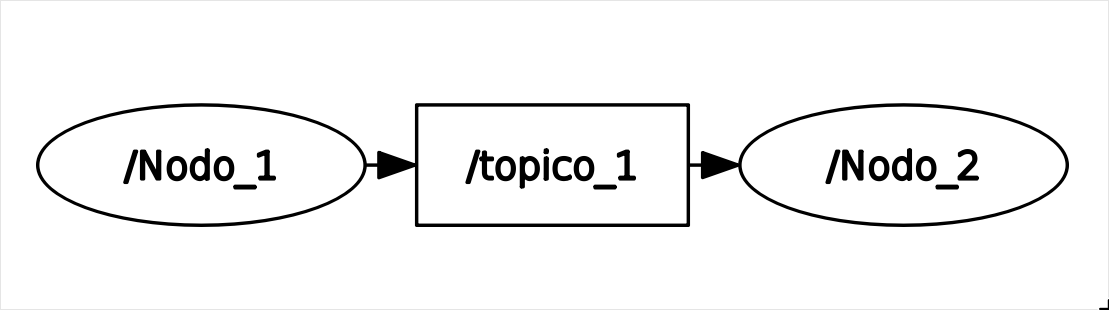
\includegraphics[width=0.5\linewidth]{images/nodo_topico.png}
    \caption{Nodos comunicados mediante un tópico}
    \label{fig:placeholder}
\end{figure}

Para desarrollar nodos se necesita de un lenguaje de programación, dependiendo
de cual se elija, el paquete será definido de manera distinta. Actualmente se
definen dos lenguajes de programación para ROS, C++ y Python. Cada uno ofrece
beneficios propios de su forma de trabajo.

% \begin{lstlisting}[language=Python, style=micode, caption={Ejemplo en Python}]
% import rclpy
% from rclpy.node import Node
% from std_msgs.msg import String

% class Nodo1(Node):
%     def __init__(self):
%         super().__init__("Nodo_1")
%         self.contador = 0
%         self.publisher_ = self.create_publisher(String, "topico_1", 10)
%         self.timer = self.create_timer(1.0, self.publicar_string)

%     def publicar_string(self):
%         msg = String()
%         msg.data = f"Hola ROS 2 #{self.contador}"
%         self.publisher_.publish(msg)
%         self.contador += 1

% def main():
%     rclpy.init()
%     nodo = Nodo1()
%     rclpy.spin(nodo)
% \end{lstlisting}

% \begin{lstlisting}[language=C++, style=micode, caption={Ejemplo en C++}]
% #include "rclcpp/rclcpp.hpp"
% #include "std_msgs/msg/string.hpp"

% class NodoPublicador : public rclcpp::Node {
% public:
%   NodoPublicador() : Node("nodo_publicador_cpp"), contador_(0) {
%     publisher = this->create_publisher<std_msgs::msg::String>("topico_1", 10);
%     timer = this->create_wall_timer(1s, std::bind(&NodoPublicador::publicar, this));
%   }

% private:
%   void publicar {
%     ...
%     publisher->publish(msg);

%   }

%   rclcpp::Publisher<std_msgs::msg::String>::SharedPtr publisher;
%   rclcpp::TimerBase::SharedPtr timer;
% };

% int main(int argc, char *argv[]) {
%   rclcpp::init(argc, argv);
%   rclcpp::spin(std::make_shared<NodoPublicador>());
%   rclcpp::shutdown();
% }
% \end{lstlisting}

%no se si deba incluir codigofuera de anexos

\subsection{Lanzadores}

Si bien los nodos y tópicos funcionan de manera que crean una red de
comunicación compleja, estos necesitan ser inicializados primero. A su vez cada
nodo puede usar una variedad de parámetros distintos o archivos de
configuración que se encuentran en otros paquetes. Para agilizar la ejecución
de sistemas más complejos se desarrollaron los paquetes lanzadores. Estos
paquetes ordenan y permiten gestionar los distintos nodos necesarios para el
funcionamiento correcto del sistema creado. Un lanzador permite llamar a los
distintos paquetes que se encuentren en el entorno de ROS, iniciar ejecutables,
llamar archivos de configuración, definir parámetros necesarios para iniciar
nodos de forma adecuada, incluso llamar a otros lanzadores.

Actualmente existen dos formas de definir un lanzador, mediante un archivo XML
o mediante Python, ambas ofrecen funciones similares bajo sus formas de
descripción y nomenclaturas.

\section{Interfaces gráficas en ROS}

La abstracción al momento de ejecutar un sistema robótico en ROS puede llegar a
dificultar la interacción con usuarios poco familiarizados con los distintos
lenguajes de programación usados en los nodos o ejecutables necesario en el
sistema a desarrollar. Bajo esta premisa se necesita una capa visual que
convierta la información del entorno de ROS a gráficas, indicadores, etc. Esta
capa visual puede ser creada en la terminal, a manera de menús con entradas de
valor o inputs y visualización de los resultados; o de forma más elaborada,
mediante un framework gráfico como Qt5 o Ctk, que permitan agregar una interfaz
más amigable e intuitiva.

Los frameworks de desarrollo son un conjunto de herramientas que permiten
construir de manera organizada una interfaz de usuario completa, permitiendo
mostrar imágenes, capturas de video, llenar formularios, etc. En el contexto de
ROS, los frameworks deben permitir ejecutar los nodos y comunicarse con ellos,
permitiendo una interacción de alto nivel entre el usuario y el sistema.

\begin{figure}[H]
    \centering
    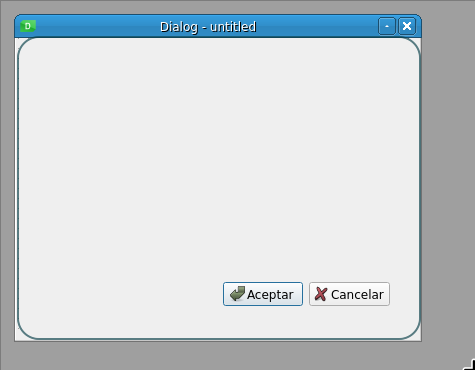
\includegraphics[width=0.5\linewidth]{images/ejemplo_interfaz.png}
    \caption{Interfaz con el framework Qt5}
    \label{fig:placeholder}
\end{figure}

\subsection{Rviz}
Rviz, ahora en su versión Rviz2, es la herramienta de visualización 3D de ROS.
Fue desarrollado para tener compatibilidad con los distintos tópicos
desarrollados en el entorno de ROS. Rviz contiene un gran conjunto de
herramientas de visualización que permiten realizar tanto análisis de
estructura o modelos de robots en 3D, como visualización de mapeos realizados
por robots móviles en planos 2D. Los tópicos gráficos que maneja Rviz incluyen
lectores de modelos URDF (Unified Robot Description Format), nube de puntos,
marcadores, árbol de transformaciones, vectores, etc.

\begin{figure}[H]
    \centering
    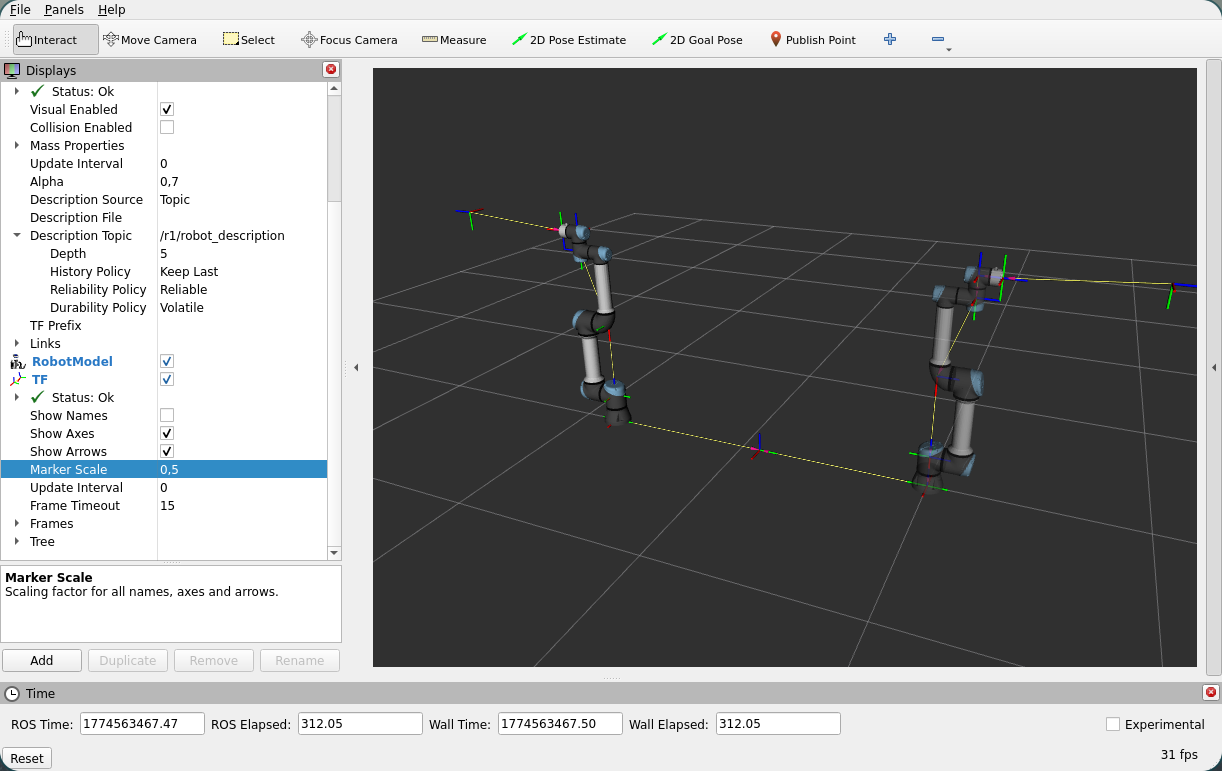
\includegraphics[width=0.75\linewidth]{images/Rviz2.png}
    \caption{Interfaz de Rviz2}
    \label{fig:placeholder}
\end{figure}

Para poder usarlo en proyectos de ROS se puede optar por abrirlo desde terminal
o incluirlo en el listado de nodos que abrirá un lanzador.

\subsection{Gazebo}
Dentro de las herramientas de simulación en ROS se encuentra Gazebo, un
simulador con alta compatibilidad de plugins e integración con los sistemas
desarrollados en el entorno de ROS. Este simulador permite replicar condiciones
físicas reales, como gravedad, colisiones, interacción entre objetos,
iluminación, visualización de sensores, etc.

Si bien no es una herramienta propia de ROS como Rviz, está desarrollada casi a
la par y muchos de los paquetes existentes se crearon para tener compatibilidad
con Gazebo, y esta a su vez desarrolla distintos complementos y herramientas
que refuerzan este vínculo.

La simulación en Gazebo permite incluir elementos como bloques, mesas, sillas y
diversas herramientas, extraídas de bibliotecas públicas, para representar de
manera realista las tareas que llevará a cabo el sistema.

\begin{figure}[H]
    \centering
    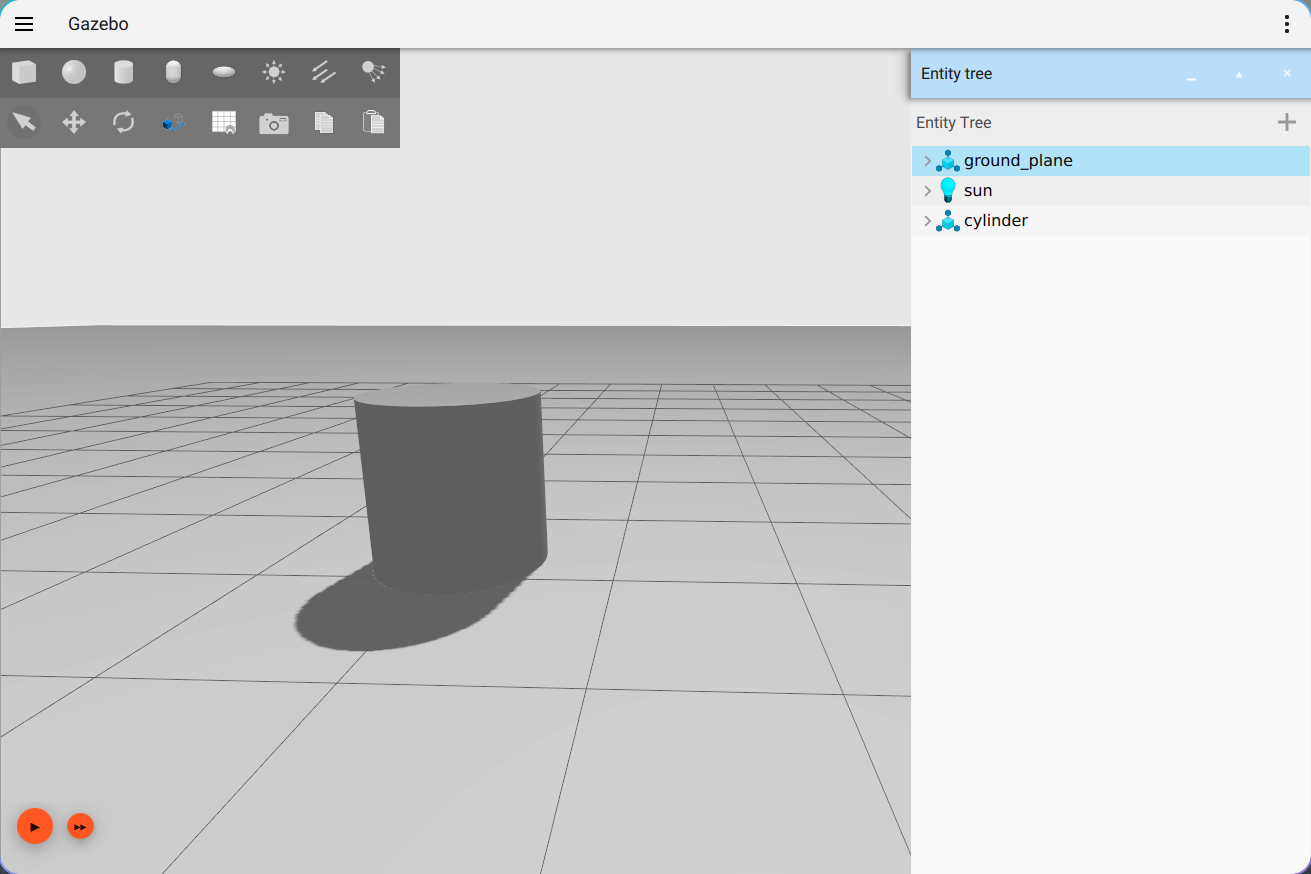
\includegraphics[width=0.75\linewidth]{images/Gazebo_ign.png}
    \caption{Entorno de Gazebo}
    \label{fig:placeholder}
\end{figure}

\subsection{Qt5}

Entre los frameworks más usados se encuentra Qt5, construido en C y con soporte
para Python, permite desarrollar interfaces multiplataformas y es la base de
las herramientas gráficas de ROS; debido a esto, se pueden crear interfaces que
tenga de manera embebida algunas de las características de las herramientas de
ROS, como es el visualizador 3D de Rviz.

Qt5 trabaja con un esquema de widgets, cada widget se puede ordenar dentro de
Layouts, estos a su vez pueden ser agregados dentro de otro widget, así
sucesivamente haciéndolo más sencillo de organizar. Adicionalmente, permite el
uso de archivos de configuración gráfica en su propio lenguaje similar a CSS,
denominado QSS.
